% !TeX program = xelatex
\documentclass[aspectratio=169,11pt]{beamer}
\usetheme{Madrid}
\usefonttheme[onlymath]{serif}
\setbeamertemplate{navigation symbols}{}
\usepackage[english]{babel}
\usepackage{amsmath,tikz}
\usepackage{animate}

\title[LevAMM]{How LevAMM targets \texorpdfstring{$2\times$}{2x} leverage}
\subtitle{From the Uniswap v2 invariant to a leverage-sensitive price}
\author{Anton Ledrov}
\institute{MIPT}
\date{\today}

\begin{document}
\begin{frame}[plain,noframenumbering]
  \titlepage
\end{frame}

\section{What does LevAMM manage?}
\definecolor{reserveRed}{HTML}{AF272E}
\definecolor{debtGreen}{HTML}{19734C}
\definecolor{collateralBlue}{HTML}{1C56A5}
\tikzset{
  market/.style={draw=structure.fg!55,fill=structure.fg!5,rounded corners=2pt,
  minimum width=2.5cm,minimum height=.8cm,align=center,font=\small},
  role/.style={font=\scriptsize,align=center},
  route/.style={->,>=stealth,thick}
}

\begin{frame}{Who funds and configures a Yield Basis market?}
  \centering
  \begin{tikzpicture}
    \node[market] (curve) at (-5,1) {Curve DAO};
    \node[market] (yb) at (-5,-1) {YB DAO};
    \node[market] (factory) at (0,0) {YB Factory\\\texttt{add\_market()}};
    \node[market,fill=structure.fg!11] (market) at (5,0)
    {cbBTC market\\[3pt]\texttt{LT} + \texttt{AMM}\\LP oracle};
    \draw[route] (curve.east) -- node[role,above,sloped]{crvUSD credit line} (factory.north west);
    \draw[route] (yb.east) -- node[role,below,sloped]{market parameters} (factory.south west);
    \draw[route] (factory) -- node[role,above]{deploys contracts} node[role,below]{allocates crvUSD} (market);
  \end{tikzpicture}

  \bigskip
  The Factory links the market to an existing cbBTC/crvUSD Curve pool.\\
  The YB DAO controls the market allocation, borrowing rate and AMM fee.

  \medskip
  {\scriptsize\href{https://gov.curve.finance/t/create-a-crvusd-credit-line-to-yield-basis/10774}{Curve DAO credit line}
  \quad$\cdot$\quad\href{https://docs.yieldbasis.com/dev/overview}{Yield Basis contract architecture}}
\end{frame}

\newcommand{\balancebar}[3]{%
  \begin{tabular}[b]{@{}c@{}}
    \textcolor{#1}{\rule{.38cm}{#2}}\\[-1pt]
    {\tiny #3}
\end{tabular}}

\begin{frame}{Where do the tokens go?}
  \centering
  \begin{tikzpicture}[scale=.92,transform shape]
    \node[market] (user) at (-5.2,2.5) {Depositor};
    \node[market] (vault) at (0,2.5) {\textbf{LT vault}};
    \node[market] (pool) at (5.2,2.5) {Curve pool\\{\tiny Fees from traders add to LP value}};
    \node[market,fill=structure.fg!12] (amm) at (0,.25) {%
      \textbf{LevAMM}\\[2pt]
      \begin{tabular}{@{}c@{\enspace\vrule\enspace}c@{}}
        {\scriptsize Before deposit} & {\scriptsize After deposit}\\[2pt]
        \balancebar{reserveRed}{14pt}{$R=C$}\,
        \balancebar{debtGreen}{1pt}{$B=0$}\,
        \balancebar{collateralBlue}{1pt}{$V=0$} &
        \balancebar{reserveRed}{9pt}{$R\downarrow$}\,
        \balancebar{debtGreen}{5pt}{$B\uparrow$}\,
        \balancebar{collateralBlue}{10pt}{$V\uparrow$}
    \end{tabular}};
    \node[market] (oracle) at (-5.2,.25) {LP oracle};
    \draw[route] ([yshift=2mm]user.east) --
    node[role,above]{cbBTC deposit} ([yshift=2mm]vault.west);
    \draw[route] ([yshift=-2mm]vault.west) --
    node[role,below]{yb-cbBTC shares} ([yshift=-2mm]user.east);
    \draw[route,reserveRed] ([xshift=-3mm]amm.north) --
    node[role,left] {\textbf{1. Draw crvUSD}} ([xshift=-3mm]vault.south);
    \draw[route,reserveRed] (vault) --
    node[role,above]{\textbf{2. Add liquidity}\\cbBTC+crvUSD} (pool);
    \draw[route,collateralBlue] (pool.south) |-
    node[role,near end,above]{\textbf{3. Mint LP tokens}} (amm.east);
    \draw[route,debtGreen,dashed] ([xshift=3mm]vault.south) --
    node[role,right]{\textbf{4. Record debt}} ([xshift=3mm]amm.north);
    \draw[route,collateralBlue,dashed] (oracle.east) --
    node[role,above]{LP price $p_0$} (amm.west);
    \node[market] (arb) at (5.2,-.6) {Arbitrageur};
    \draw[route,<->,black!65] (amm.east |- arb.west) --
    node[role,above]{LP/crvUSD} (arb.west);
    \node[role,collateralBlue,below=4pt] at (amm.south)
    {Collateral value $V=p_0Q$};
  \end{tikzpicture}

  \par\smallskip
  {\scriptsize\href{https://docs.yieldbasis.com/user/introduction}
  {Unstaked shares earn net trading fees. Staked shares earn YB rewards.}}
\end{frame}

\begin{frame}{What does LevAMM manage?}
  \begin{columns}[c,onlytextwidth]
    \begin{column}{.58\textwidth}
      \begin{tabular}{@{}ll@{}}
        \structure{\Large $R$} & \textbf{Available reserve}\\
        & crvUSD available to lend.\\[.65em]
        \structure{\Large $V$} & \textbf{Collateral value}\\
        & $Q$ LP tokens at price $p_0$: $V=p_0Q$.\\[.65em]
        \structure{\Large $B$} & \textbf{Outstanding debt}\\
        & crvUSD borrowed against the collateral.
      \end{tabular}
    \end{column}
    \begin{column}{.36\textwidth}
      {\small Credit capacity: $C=R+B=\text{const}$}\par\smallskip
      \href{https://github.com/yield-basis/yb-core/blob/master/contracts/AMM.vy\#L439-L445}
      {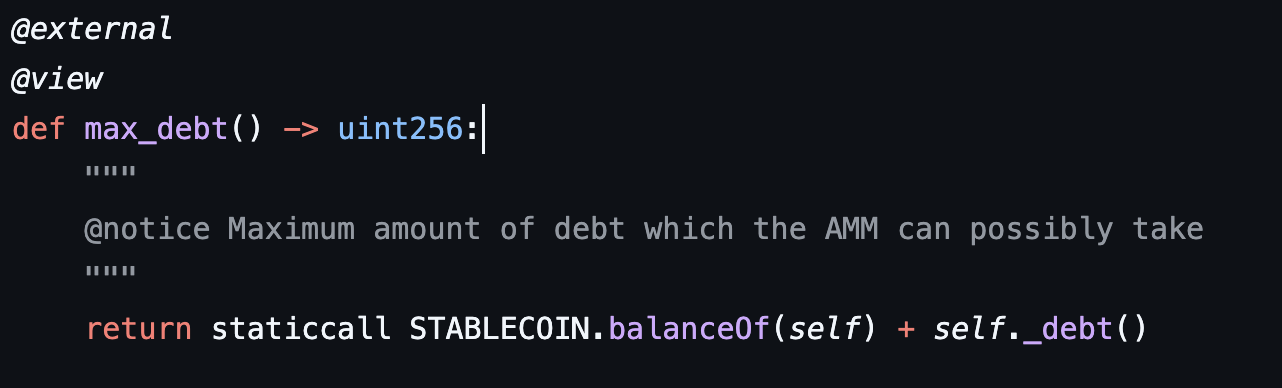
\includegraphics[width=\linewidth]{figures/max-debt.png}}\par
      {\scriptsize\color{black!60}\href{https://github.com/yield-basis/yb-core/blob/master/contracts/AMM.vy\#L439-L445}{Contract source: \texttt{AMM.vy}, \texttt{max\_debt()}}}
    \end{column}
  \end{columns}
  \bigskip
  At fixed $C$ and $p_0$, these balances describe the whole market:
  \begin{equation}\label{eq:market-state}
    (Q,B)\quad\longmapsto\quad (R,V,B)=(C-B,\ p_0Q,\ B).
  \end{equation}

  \vspace{-1em}

  \begin{block}{What does a depositor own?}
    LT issues yb-LP shares. Holding a fraction $\alpha$ of the shares gives
    exposure to $\alpha(V-B)$ of market equity. The unused credit $R$ stays
    available for future borrowing.
  \end{block}
\end{frame}

\begin{frame}{Why target $2\times$ leverage?}
  \centering
  {\large Small price moves, in percent}
  \[
    \underbrace{\text{cbBTC}}_{\text{asset price}}
    \quad\xrightarrow{\;\times\,\tfrac12\;}\quad
    \underbrace{\text{LP}}_{\text{square-root exposure}}
    \quad\xrightarrow{\;\times\,2\;}\quad
    \underbrace{\text{Equity}}_{\text{same gain on half the capital}}
  \]
  \medskip
  \structure{\textbf{At $2\times$, equity moves one-for-one with cbBTC.}}

  \bigskip
  {\scriptsize Frictionless model, \eqref{eq:app-lp-elasticity}--\eqref{eq:app-equity-elasticity}. \href{https://docs.yieldbasis.com/user/economics/math-primer}{Yield Basis Math Primer, \S\S1--2}}
\end{frame}

\section{How should the pool quote?}
\begin{frame}{Quick primer about the pool's marginal price $m$}
  \begin{columns}[c,onlytextwidth]
    \begin{column}{.53\textwidth}
      Suppose the pool holds $x$ apples and $y$ bananas.
      A trader gives it apples ($\Delta x>0$) and receives bananas ($\Delta y<0$).
      \begin{equation}\label{eq:marginal-definition}
        \underbrace{\frac{-\Delta y}{\Delta x}}_{\text{bananas per apple}}
        \quad\xrightarrow{\ \Delta x\to 0\ }\quad
        m=-\frac{\mathrm dy}{\mathrm dx}.
      \end{equation}
    \end{column}
    \begin{column}{.43\textwidth}
      \ifdefined\FermatFruit
      \centering
      {\usebeamercolor[fg]{structure}\bfseries Fermat's Last Fruit Theorem}\par
      \smallskip
      {\small For any positive whole numbers of apples and bananas, and any integer $n>2$,}
      \[
        \sqrt[n]{%
          \vphantom{A}\raisebox{-.2em}{
\includegraphics[height=1.45em]{figures/apple.png}}^{n}
          +
          \vphantom{A}\raisebox{-.2em}{
\includegraphics[height=1.45em]{figures/banana.png}}^{n}
        }\notin\mathbb{N}.
      \]
      {\scriptsize\itshape The proof won't fit in this margin.}
      \else
      
\includegraphics[width=\linewidth]{figures/fruit-puzzle-captioned.png}
      \fi
    \end{column}
  \end{columns}

  \begin{block}{For our pool}
    Replace apples with LP tokens ($x=Q$) and bananas with crvUSD ($y=R$).
    \begin{equation}\label{eq:marginal-crvusd}
      m=-\frac{\mathrm dR}{\mathrm dQ}
      \qquad \text{crvUSD paid per LP token.}
    \end{equation}
  \end{block}
  The oracle quotes $p_0$ in the same units, so we can compare the two prices.
\end{frame}

\begin{frame}{Where should arbitrage stop?}
  Equity is the part of the collateral value left after repaying the debt:
  \begin{equation}\label{eq:leverage-definition}
    E=V-B,\qquad L=\frac{V}{E}=\frac{V}{V-B}.
  \end{equation}
  \begin{block}{The design requirement}
    Arbitrage should run out of spread precisely when debt equals equity:
    \begin{equation}\label{eq:design-target}
      \underbrace{m=p_0}_{\text{no marginal arbitrage}}
      \quad\Longleftrightarrow\quad
      \underbrace{V=2B}_{L=2}.
    \end{equation}
  \end{block}
  We hold $p_0$ fixed and ignore fees.
\end{frame}

\begin{frame}{What about the Uniswap v2?}
  For the constant-product curve $RQ=k$, the slope gives $m=-\mathrm dR/\mathrm dQ=R/Q$.
  \begin{equation}\label{eq:unshifted-parity}
    \underbrace{m=p_0}_{\text{arbitrage stops}}
    \quad\Longleftrightarrow\quad
    \underbrace{R=p_0Q=V}_{\text{equal reserve values}}.
  \end{equation}

  \begin{block}{The $2\times$ leverage condition}
    The position has $2\times$ leverage when $V=2B$.
    At price parity, this would require $R=2B$ as well.
  \end{block}

  Price parity fixes $R/Q=p_0$. The debt $B$ does not enter that condition.

  \medskip
  {\scriptsize\href{https://app.uniswap.org/whitepaper.pdf}{Uniswap v2 Core, \S2.2}}
\end{frame}

\begin{frame}{Keep the constant product. Choose its two reserves.}
  \begin{columns}[c,onlytextwidth]
    \begin{column}{.62\textwidth}
      We keep the CPMM invariant $xy=I$. For LevAMM, choose
      \begin{equation}\label{eq:reserve-choice}
        \underbrace{x=Q}_{\text{Curve LP tokens held}}
        \qquad
        \underbrace{y=f(R)}_{\text{virtual crvUSD reserve}}.
      \end{equation}
      Here $R$ is the actual crvUSD balance. At fixed credit capacity $C$,
      the debt $B$ determines it through $R=C-B$.
    \end{column}
    \begin{column}{.34\textwidth}
      \animategraphics[autoplay,loop,poster=first,width=\linewidth]{15}{figures/livesey-frames/frame-}{01}{14}
    \end{column}
  \end{columns}

  \medskip
  \begin{block}{The invariant and the slope in virtual reserves}
    \begin{equation}\label{eq:virtual-cpmm}
      f(R)\,Q=I
      \qquad\qquad
      m=-\left.\frac{\mathrm dy}{\mathrm dx}\right|_I
      =\frac{y}{x}=\frac{f(R)}{Q}.
    \end{equation}
  \end{block}
\end{frame}

\begin{frame}{How should the virtual crvUSD reserve $f(R)$ be chosen?}
  Use $y=f(R)$ in the constant product $f(R) \cdot Q=I$. Two requirements guide the choice.

  \begin{block}{During a swap: match the actual crvUSD transfer}
    When crvUSD enters or leaves the pool, the virtual reserve moves
    by exactly the same amount as the actual reserve:
    \begin{equation}\label{eq:shift-condition}
      \boxed{\mathrm df=\mathrm dR}.
    \end{equation}
  \end{block}

  \begin{block}{At the leverage target: close the arbitrage spread}
    When debt is half the collateral value, the pool must quote the oracle price:
    \begin{equation}\label{eq:parity-condition}
      \boxed{V=2B=2(C-R) \quad\Longrightarrow\quad m=\frac{f(R)}{Q}=p_0}.
    \end{equation}
  \end{block}
\end{frame}

\begin{frame}{The virtual reserve is a shifted crvUSD balance}
  The virtual and actual reserves move together, so their difference is constant:
  \begin{equation}\label{eq:reserve-shift}
    \mathrm d(f-R)=0
    \quad\Longrightarrow\quad \boxed{f(R)=R+s}.
  \end{equation}
  The shift $s$ stays fixed along a swap curve. With $R=C-B$ and $x_0=C+s$,
  the same invariant can be written in terms of debt:
  \begin{equation}\label{eq:shifted-invariant}
    (R+s)Q=\boxed{(x_0-B)Q=I}.
    \qquad ((\text{\scriptsize\color{structure.fg}\href{https://docs.yieldbasis.com/user/economics/math-primer}{YB Math Primer, Eq.~(3.2)}}))
  \end{equation}
  \begin{block}{The price paid in actual crvUSD}
    Along this curve, $Q\,\mathrm dB=(x_0-B)\,\mathrm dQ$, so
    \begin{equation}\label{eq:shifted-price}
      m=-\frac{\mathrm dR}{\mathrm dQ}
      =\frac{\mathrm dB}{\mathrm dQ}=\frac{x_0-B}{Q}.
    \end{equation}
  \end{block}
\end{frame}

\begin{frame}{Which point on the swap curve are we looking for?}
  \centering
  \begin{tikzpicture}[>=stealth]
    \draw[fill=collateralBlue!5,draw=collateralBlue!45,rounded corners=3pt]
    (-6.4,1.45) rectangle (-.45,3.75);
    \draw[fill=debtGreen!5,draw=debtGreen!45,rounded corners=3pt]
    (.45,1.45) rectangle (6.4,3.75);

    \node[collateralBlue,font=\bfseries] at (-3.425,3.37) {Price matches the oracle};
    \node[font=\Large] at (-3.425,2.60) {$m_*=p_0$};
    \node[font=\footnotesize] at (-3.425,1.87) {No marginal arbitrage};

    \node[debtGreen,font=\bfseries] at (3.425,3.37) {Leverage is $2\times$};
    \fill[debtGreen!24] (1.02,2.29) rectangle (3.425,2.93);
    \fill[debtGreen!9] (3.425,2.29) rectangle (5.83,2.93);
    \draw[debtGreen!70] (1.02,2.29) rectangle (5.83,2.93);
    \draw[debtGreen!70] (3.425,2.29) -- (3.425,2.93);
    \node[font=\small] at (2.22,2.61) {Debt $B_*$};
    \node[font=\small] at (4.63,2.61) {Equity $E_*$};
    \node[font=\footnotesize] at (3.425,1.87) {Equal halves of collateral value $V_*$};

    \node[market,fill=structure.fg!12,minimum width=4.3cm] (target) at (0,.05)
    {\textbf{Target point} $(Q_*,B_*)$};
    \draw[route,collateralBlue] (-3.425,1.45) -- ([xshift=-1.1cm]target.north);
    \draw[route,debtGreen] (3.425,1.45) -- ([xshift=1.1cm]target.north);
  \end{tikzpicture}

  \medskip
  {\small\color{black!65}
    The \href{https://docs.yieldbasis.com/user/economics/math-primer\#ideal-debt-at-the-oracle-price}
  {\structure{Math Primer}} writes $Q_*$ and $B_*$ as $\tilde y$ and $\tilde d$.}
\end{frame}

\begin{frame}{Which balances satisfy both conditions?}
  \textbf{Price.} At $(Q_*,B_*)$, the pool quotes the oracle price:
  \begin{equation}\label{eq:target-price}
    m_*=\frac{x_0-B_*}{Q_*}=p_0
    \quad\Longrightarrow\quad x_0-B_*=p_0Q_*=V_*.
  \end{equation}
  \textbf{Leverage.} Divide collateral value by equity and set the ratio to two:
  \begin{equation}\label{eq:target-leverage}
    L_*=\frac{V_*}{V_*-B_*}=2
    \ \Longrightarrow\ V_*=2(V_*-B_*)
    \ \Longrightarrow\ V_*=2B_*.
  \end{equation}

  \begin{equation}\label{eq:target-balances}
    \begin{cases}
      x_0-B_*=p_0Q_*,\\
      p_0Q_*=2B_*
    \end{cases}
    \quad\Longrightarrow\quad
    \boxed{B_*=\frac{x_0}{3},\qquad Q_*=\frac{2x_0}{3p_0}.}
  \end{equation}
\end{frame}

\begin{frame}{Which invariant passes through that point?}
  On a given swap curve, $(x_0-B)Q=I$ at every point. Its value at the
  target balances must therefore be the same $I$:
  \begin{equation}\label{eq:calibrated-invariant}
    I=(x_0-B_*)Q_*
    =\left(x_0-\frac{x_0}{3}\right)\frac{2x_0}{3p_0}
    =\frac{2x_0}{3}\frac{2x_0}{3p_0}
    =\boxed{\frac{4x_0^2}{9p_0}}.
  \end{equation}
  \begin{block}{Back to the current balances $(Q,B)$}
    We have used the target to fix the relation between $I$ and $x_0$.
    The current balances must lie on that same curve:
    \begin{equation}\label{eq:current-invariant}
      (x_0-B)Q=\frac{4x_0^2}{9p_0}.
    \end{equation}
  \end{block}
\end{frame}

\begin{frame}{Which curve passes through today's position?}
  Given debt $B$ and collateral value $V=p_0Q$, solve for $x_0$:
  \begin{equation}\label{eq:anchor-quadratic}
    (x_0-B)Q=\frac{4x_0^2}{9p_0}
    \quad\Longrightarrow\quad
    \frac49x_0^2-Vx_0+VB=0.
  \end{equation}
  \begin{equation}\label{eq:anchor-roots}
    x_0^\pm=\frac98\!\left(V\pm\sqrt{V^2-\tfrac{16}{9}VB}\right).
  \end{equation}
  \begin{block}{$x_0^+$ or $x_0^-$?}
    \begin{equation}\label{eq:roots-at-target}
      x_0^+=\tfrac32 V_*,\qquad x_0^-=\tfrac34 V_*.
    \end{equation}
    \begin{equation}\label{eq:branch-choice}
      \frac{m_*}{p_0}=\frac{x_0-B_*}{V_*}
      =
      \begin{cases}
        \tfrac32-\tfrac12=\textcolor{structure.fg}{\boxed{1}} & (+),\\
        \tfrac34-\tfrac12=\tfrac14 & (-).
      \end{cases}
    \end{equation}
  \end{block}
\end{frame}

\section{The arbitrage trade}
\begin{frame}{The debt share determines the price gap}
  The debt share $r=B/V$ is the fraction of collateral value financed by debt.
  \begin{equation}\label{eq:debt-share}
    L=\frac{V}{V-B}=\frac{1}{1-r},
    \qquad r=\tfrac12\ \Longleftrightarrow\ L=2.
  \end{equation}
  The normalized quote uses the plus branch of \eqref{eq:app-normalized-quote} at $\ell=2$:
  \begin{equation}\label{eq:normalized-quote}
    F(r)=\frac{m}{p_0}=\frac98\!\left(1+\sqrt{1-\tfrac{16}{9}r}\right)-r,
    \qquad 0\le r\le\tfrac{9}{16}.
  \end{equation}
  \begin{columns}[c,onlytextwidth]
    \begin{column}{.54\textwidth}
      \centering
      \begin{tikzpicture}[x=41cm,y=3.4cm,>=stealth,font=\scriptsize]
        % Horizontal coordinates are measured relative to the target r=1/2.
        \draw[->] (-.086,0) -- (.076,0) node[below right] {$r$};
        \draw[->] (-.082,-.46) -- (-.082,.38) node[right] {Price gap $m/p_0-1$};
        \node[left] at (-.082,0) {$0$};
        \draw[structure.fg,very thick,domain=0:.5,samples=65,variable=\t]
        plot ({9/16*(1-\t*\t)-.5},{9/8*(1+\t)-9/16*(1-\t*\t)-1});
        \draw[->,line width=1.5pt,structure.fg] (-.063,0) -- (-.012,0);
        \draw[->,line width=1.5pt,structure.fg] (.055,0) -- (.012,0);
        \fill (0,0) circle (1.7pt) node[below left] {$1/2$};
        \draw[dotted,gray] (.0625,0)--(.0625,-.4375);
        \node[above] at (.0625,0) {$9/16$};
      \end{tikzpicture}
    \end{column}
    \begin{column}{.43\textwidth}
      \textbf{Left of the target: $m>p_0$.}\\
      Traders sell LP to the pool. Its quote falls toward $p_0$ and $r$ rises.

      \medskip
      \textbf{Right of the target: $m<p_0$.}\\
      Traders buy LP from the pool. Its quote rises toward $p_0$ and $r$ falls.
    \end{column}
  \end{columns}

  \medskip
  \centering At $r=1/2$, the spread vanishes: $m=p_0$ and leverage is $2\times$.
\end{frame}

\begin{frame}{Final takeaway}
  \centering
  \setlength{\fboxsep}{7pt}
  {\Large\fbox{\strut LevAMM is just a shifted uniV2 with properly configured parameters.}\par}

  \bigskip
  In the fee-free model, arbitrage moves debt toward half the collateral value.
  \begin{equation}\label{eq:final-takeaway}
    \boxed{m=p_0\quad\Longleftrightarrow\quad
    \frac{B}{V}=\frac12\quad\Longleftrightarrow\quad L=2.}
  \end{equation}
\end{frame}

\appendix
\section{Derivations for arbitrary target leverage}
\setcounter{equation}{0}
\renewcommand{\theequation}{A.\arabic{equation}}
\renewcommand{\theHequation}{appendix.\arabic{equation}}

\begin{frame}{Appendix. Why an LP has half the price exposure}
  Use a fee-free constant-product benchmark for the Curve LP.
  Let $a,b>0$ be the cbBTC and crvUSD reserves. Arbitrage sets
  $P=b/a$, where $P$ is the cbBTC price in crvUSD. The product $ab=k$
  stays fixed as the price moves. Write $L=V/(V-B)$ for current leverage
  and $\ell>1$ for the target.
  \begin{equation}\label{eq:app-lp-reserves}
    a=\sqrt{k/P},\qquad b=\sqrt{kP}.
  \end{equation}

  For a fixed LP ownership fraction $\theta$, the collateral is worth
  $\theta$ times the reserve value. Substituting \eqref{eq:app-lp-reserves}
  gives
  \begin{equation}\label{eq:app-lp-value}
    V(P)=\theta(Pa+b)=2\theta\sqrt{kP}.
  \end{equation}
  Take the logarithmic derivative at fixed $\theta$ and $k$:
  \begin{equation}\label{eq:app-lp-elasticity}
    \frac{\mathrm dV}{V}=\frac12\frac{\mathrm dP}{P}.
  \end{equation}
\end{frame}

\begin{frame}{Appendix. Equity exposure at constant leverage}
  Start with equity $E=V-B>0$ and leverage $L=V/E$ from
  \eqref{eq:leverage-definition}. During a small price move with debt fixed,
  $\mathrm dE=\mathrm dV$: equity takes the entire gain or loss on the collateral.
  Divide by $E$ and apply \eqref{eq:app-lp-elasticity}:
  \begin{equation}\label{eq:app-equity-elasticity}
    \frac{\mathrm dE}{E}
    =\frac{V}{E}\frac{\mathrm dV}{V}
    =\frac{L}{2}\frac{\mathrm dP}{P}.
  \end{equation}

  In the idealized continuous-rebalancing model, each resize is funded
  by an equal change in debt, so the resize leaves equity unchanged.
  With $L=\ell$ along a smooth price path and zero fees and costs, integrate
  \eqref{eq:app-equity-elasticity} from $P_{\mathrm{start}}$:
  \begin{equation}\label{eq:app-equity-path}
    \log\frac{E(P)}{E(P_{\mathrm{start}})}
    =\frac{\ell}{2}\log\frac{P}{P_{\mathrm{start}}}
    \quad\Longrightarrow\quad
    E(P)=E(P_{\mathrm{start}})\left(\frac{P}{P_{\mathrm{start}}}\right)^{\ell/2}.
  \end{equation}
  At $\ell=2$, the exponent is one, so equity tracks the cbBTC price.
\end{frame}

\begin{frame}{Appendix. From a marginal trade to price parity}
  On a smooth, fee-free swap curve, selling $\mathrm dQ>0$ LP tokens
  pays out $-\mathrm dR$ crvUSD. This gives \eqref{eq:marginal-definition}
  and \eqref{eq:marginal-crvusd}. If the LP can be traded externally at
  $p_0$, the marginal profit is
  \begin{equation}\label{eq:app-marginal-profit}
    \mathrm d\Pi=(m-p_0)\,\mathrm dQ.
  \end{equation}
  With both trade directions available, a positive spread favours selling
  LP to the pool and a negative spread favours buying it. Neither side
  earns a positive marginal profit at $m=p_0$.

  On the unshifted curve $RQ=k$, differentiating with $k$ fixed gives
  \begin{equation}\label{eq:app-unshifted-price}
    Q\,\mathrm dR+R\,\mathrm dQ=0
    \quad\Longrightarrow\quad
    m=-\frac{\mathrm dR}{\mathrm dQ}=\frac{R}{Q}.
  \end{equation}
  Thus parity gives $R=p_0Q=V$ as in \eqref{eq:unshifted-parity}.
  The leverage target additionally requires $B/V=1-1/\ell$ by
  \eqref{eq:leverage-definition}.
\end{frame}

\begin{frame}{Appendix. From the reserve shift to the swap quote}
  For the choice \eqref{eq:reserve-choice}, differentiating $f(R)Q=I$
  along one curve gives the virtual slope in \eqref{eq:virtual-cpmm}:
  \begin{equation}\label{eq:app-virtual-slope}
    Q\,\mathrm df+f(R)\,\mathrm dQ=0
    \quad\Longrightarrow\quad
    -\frac{\mathrm df}{\mathrm dQ}=\frac{f(R)}{Q}.
  \end{equation}
  Requiring this slope to equal the actual cash quote
  $-\mathrm dR/\mathrm dQ$ yields $\mathrm df=\mathrm dR$
  in \eqref{eq:shift-condition}. Integrating on a connected swap curve
  gives $f(R)=R+s$ as in \eqref{eq:reserve-shift}.

  With $R=C-B$ and $x_0=C+s$, this gives \eqref{eq:shifted-invariant}.
  Differentiating with $x_0,I,C$ fixed yields
  \begin{equation}\label{eq:app-shifted-price}
    Q\,\mathrm dB=(x_0-B)\,\mathrm dQ
    \quad\Longrightarrow\quad
    m=\frac{\mathrm dB}{\mathrm dQ}=\frac{x_0-B}{Q}.
  \end{equation}
\end{frame}

\begin{frame}{Appendix. Calibrating at arbitrary target leverage}
  At fixed $p_0>0$, take $x_0>0$ and set $L_*=\ell>1$. The target
  is at price parity and has debt share $r_*=B_*/V_*$:
  \begin{align}
    m_*=p_0 &\Longrightarrow x_0-B_*=p_0Q_*=V_*,
    \label{eq:app-target-price}\\
    \frac{V_*}{V_*-B_*}=\ell &\Longrightarrow
    B_*=r_*V_*,\qquad r_*=1-\frac1\ell.
    \label{eq:app-target-leverage}
  \end{align}
  Combining the two conditions gives $x_0=(1+r_*)V_*$. Hence
  \begin{equation}\label{eq:app-target-balances}
    B_*=\frac{\ell-1}{2\ell-1}\,x_0,\qquad
    Q_*=\frac{\ell}{2\ell-1}\,\frac{x_0}{p_0}.
  \end{equation}
  Substitute $x_0-B_*=V_*=p_0Q_*$ into the invariant:
  \begin{equation}\label{eq:app-calibration}
    I=p_0Q_*^2=\lambda\frac{x_0^2}{p_0},
    \qquad \lambda=\left(\frac{\ell}{2\ell-1}\right)^2
    =\frac{1}{(1+r_*)^2}.
  \end{equation}
\end{frame}

\begin{frame}{Appendix. Solving for the anchor at the observed state}
  The same curve passes through the observed $(Q,B)$. Insert
  \eqref{eq:app-calibration} into $(x_0-B)Q=I$ and multiply by $p_0$.
  With $V=p_0Q$, this gives
  \begin{equation}\label{eq:app-quadratic}
    (x_0-B)V=\lambda x_0^2
    \quad\Longleftrightarrow\quad
    \lambda x_0^2 - Vx_0 + VB=0.
  \end{equation}
  The quadratic formula gives
  \begin{equation}\label{eq:app-discriminant}
    D=V^2-4\lambda VB,\qquad
    x_0^\pm=\frac{V\pm\sqrt D}{2\lambda}.
  \end{equation}
  With $V>0$ and $B\ge 0$, the real-root domain is
  \begin{equation}\label{eq:app-domain}
    D=V^2(1-4\lambda r)\ge0
    \quad\Longleftrightarrow\quad
    0\le r=\frac BV\le\frac{1}{4\lambda}.
  \end{equation}
  At $\ell=2$, $\lambda=4/9$ and the upper bound is $9/16$.
\end{frame}

\begin{frame}{Appendix. Choosing the branch at arbitrary leverage}
  At $r=r_*$, use $\lambda=1/(1+r_*)^2$ from \eqref{eq:app-calibration}:
  \begin{equation}\label{eq:app-target-discriminant}
    \frac{\sqrt{D_*}}{V_*}
    =\sqrt{1-\frac{4r_*}{(1+r_*)^2}}
    =\frac{1-r_*}{1+r_*},
    \qquad 0<r_*<1.
  \end{equation}
  Substituting into \eqref{eq:app-discriminant} gives
  \begin{equation}\label{eq:app-roots-at-target}
    \frac{x_0^+}{V_*}=1+r_*,
    \qquad
    \frac{x_0^-}{V_*}=r_*(1+r_*).
  \end{equation}
  Evaluate the price on each root using \eqref{eq:app-shifted-price}:
  \begin{equation}\label{eq:app-branch}
    \frac{m_*^\pm}{p_0}=\frac{x_0^\pm}{V_*}-r_*
    =
    \begin{cases}
      1 & (+),\\
      r_*^2 & (-).
    \end{cases}
  \end{equation}
  The plus root gives the required $m_*=p_0$ because $r_*^2<1$.
\end{frame}

\begin{frame}{Appendix. How the price signals a leverage deviation}
  Divide the plus root in \eqref{eq:app-discriminant} by $V$ and use
  \eqref{eq:app-shifted-price}:
  \begin{equation}\label{eq:app-normalized-quote}
    F_\ell(r)=\frac{m}{p_0}=\frac{x_0^+}{V}-r
    =\frac{1+\sqrt{1-4\lambda r}}{2\lambda}-r.
  \end{equation}
  The spread vanishes at $r_*=1-1/\ell$ by \eqref{eq:app-branch}.
  On the interior of the domain in \eqref{eq:app-domain},
  \begin{equation}\label{eq:app-monotonicity}
    F_\ell(r_*)=1,\qquad
    F_\ell'(r)=-1-\frac{1}{\sqrt{1-4\lambda r}}<0.
  \end{equation}
  The debt share determines current leverage:
  \begin{equation}\label{eq:app-leverage-from-debt}
    L=\frac1{1-r},\qquad r=r_* \Longleftrightarrow L=\ell.
  \end{equation}
  Thus the AMM quotes a premium below the leverage target and a discount above it.
\end{frame}

\begin{frame}{Appendix. Why arbitrage moves toward any leverage target}
  At fixed $p_0$, differentiate $r=B/(p_0Q)$ and use
  $\mathrm dB=m\,\mathrm dQ$ from \eqref{eq:app-shifted-price}:
  \begin{equation}\label{eq:app-phase}
    \mathrm dr=\bigl(F_\ell(r)-r\bigr)\frac{\mathrm dQ}{Q},
    \qquad
    F_\ell(r)-r=\frac{1+\sqrt{1-4\lambda r}}{2\lambda}-2r>0
    \quad\left(0\le r<\frac1{4\lambda}\right).
  \end{equation}
  Since $2r<1/(2\lambda)$ in the interior, $r$ moves in the same direction
  as $Q$. Combine this with the profit signal \eqref{eq:app-marginal-profit}:
  \begin{align}
    r<r_* &\Longrightarrow m>p_0
    \Longrightarrow \text{sell LP to the AMM}
    \Longrightarrow \mathrm dQ>0,\ \mathrm dr>0,\label{eq:app-sell}\\
    r>r_* &\Longrightarrow m<p_0
    \Longrightarrow \text{buy LP from the AMM}
    \Longrightarrow \mathrm dQ<0,\ \mathrm dr<0.\label{eq:app-buy}
  \end{align}
  With both trade directions available, this moves leverage toward $\ell$ locally.
\end{frame}

\end{document}
